%%
%% 研究報告用スイッチ
%% [techrep]
%%
%% 欧文表記無しのスイッチ(etitle,eabstractは任意)
%% [noauthor]
%%

%\documentclass[submit,techrep]{ipsj}
\documentclass[submit,techrep,noauthor]{ipsj}
\usepackage[dvipdfmx]{graphicx}
\usepackage{latexsym}
\usepackage{comment}
\usepackage{here}
\usepackage{cite}
\usepackage{url}




\def\Underline{\setbox0\hbox\bgroup\let\\\endUnderline}
\def\endUnderline{\vphantom{y}\egroup\smash{\underline{\box0}}\\}
\def\|{\verb|}
%

%\setcounter{巻数}{59}%vol59=2018
%\setcounter{号数}{10}
%\setcounter{page}{1}


\begin{document}

\title{ヒュージページを活用する\\インメモリ分散処理フレームワーク}
%\etitle{An in-memory distributed processing framework that utilizes hugepage}

\affiliate{tuat}{東京農工大学\\
Tokyo University of Agriculture and Technology}

\author{宮里 勇也}{Yuya Miyazato}{tuat}
\author{山田 浩史}{Hiroshi Yamada}{tuat}


\begin{abstract}
  分散処理システムとは,複数のコンピュータで処理を分散して行うシステムで,大規模なデータを
  処理することができ,サーバのコスト削減やリソースの拡張性といったメリットが存在する.
  中でもApache Sparkのようなインメモリ分散処理フレームワークでは,処理を出来る限り
  メモリ内で行うことで,従来のものよりも高速な処理が可能となる.
  インメモリ分散処理では膨大なデータをメモリ上で扱う都合上,アドレス変換が大きなボトルネックになってしまう.
  アドレス変換のボトルネックを解消する機構としてヒュージページがある.
  Apache Sparkにヒュージページを適用する場合,主にTHPというヒュージページ管理機構が
  用いられるが,THPにはメモリ肥大化や,メモリのコンパクションのためにCPUが占有されるなど様々な問題が
  存在している.
  Apache SparkにおいてもTHPによるヒュージページ割り当ての効果は大きいが,THPのデメリットも受けてしまうため
  闇雲にヒュージページを利用することはできない.  
  本研究ではインメモリ分散処理フレームワーク上でヒュージページを効率的に利用できる手法を提案する.
  提案方式では,Apache Sparkのデータ領域の中でも,ヒュージページの効果が大きい領域にのみ
  ヒュージページの割り当てを行い,それ以外では通常のページ割り当てを行うことで無駄なヒュージページ割り当てを避ける.
  これにより,メモリ肥大化やコンパクションなどのデメリットを抑えつつ,ヒュージページによる性能向上の恩恵を受けることを狙う.
  実験の結果,  マイクロベンチマークのようなキャッシュデータへのアクセス頻度が高い
  ワークロードでは一部のみのヒュージページ割り当てで全体割り当てと同等以上のパフォーマンスが得られた.
\end{abstract}

%% キーワード (1--5単語) の記載は任意.
\begin{jkeyword}
分散処理システム,ヒュージページ
\end{jkeyword}

%\begin{eabstract}
%\end{eabstract}

%% the following keyword part is optional and can be omitted.

%\begin{ekeyword}
%  System security
%\LaTeX, style files
%\end{ekeyword}

%% if you use english opsion, you should put your English abstract in the abstract environment.
%% eabstract is not displayed in english mode


\maketitle

\section{はじめに} \label{section:introduction}
Spark に代表されるインメモリ分散処理フレームワーク~\cite{zaharia2010spark}は,マシンに搭載されている膨大なメモリを活用するアプリケーションを構築するフレームワークである.インメモリ分散処理フレームワークは分散処理フレームワーク\cite{dean2008mapreduce}の一種で,各マシン内での処理を可能な限りメモリ内で行うことで,巨大なメモリを要するアプリケーションの実現やストレージ I/O を抑えながらの処理速度向上が期待できる.たとえば,巨大なグラフを解析したり,大量のデータを必要とする機械学習などのアプリケーションの実現に利用される.インメモリ分散処理フレームワークにおいて膨大なメモリが必要な理由として,通常の分散処理フレームワークとの処理方式の違いが挙げられる.分散処理フレームワークでは,データの処理を行うたびにストレージへの書き出しを行う.対して,インメモリ分散処理フレームワークでは,データの処理が終わった後,ディスクへの書き出しを行わず,そのままメモリ内に保持し続けることで処理の高速化を実現している.このデータを保持するために膨大なメモリが必要となる.実際に多くのメモリを搭載するマシンの例として,Amazon EC2 が提供するHigh Memory インスタンス\cite{amazon-ec2-high-memory}では,最大24TBものメモリを搭載しており,この巨大なサイズのメモリをインメモリ分散処理フレームワークなどのアプリケーションが利用することになる.

インメモリ分散処理フレームワークなどの膨大なメモリを利用するアプリケーションでは,アドレス変換が大きなボトルネックとなることが知られている~\cite{basu2013efficient, gandhi2014efficient}.メモリ管理にはページングが広く利用されており,ページという単位で仮想アドレスと物理アドレスの変換を行う.高速化のために一度変換したページは TLB という高速なハードウェアに保存することでアドレス変換を高速に行うことが可能となるが,TLBはサイズがあまり大きくない.そのため,膨大なメモリに対してはTLBにキャッシュしておける量が少なくなり,TLBを使ってアドレス変換できる範囲が狭く,多くのアドレス変換は TLB を使わない遅いものとなってしまう.

このような問題点を解決するために,ヒュージページという機構が存在する.ヒュージページでは,ページのサイズを通常よりも大きいサイズで使用することで一度に変換できるアドレスの範囲を大きくすることができる.これによってTLB に保存できるアドレスの範囲が増え,多くのページで高速なアクセスが可能となり,他にもページテーブルサイズの削減やページウォーク時間の短縮といった効果が得られる.

インメモリ分散処理フレームワークでは膨大なメモリを利用することから,ヒュージページの恩恵を期待できる.しかし,インメモリ分散処理フレームワークにヒュージページを適用する研究は存在しおらず,効率的なヒュージページの使用法はわかっていない.また,インメモリ分散処理フレームワークでヒュージページを適用するのはアプリケーション単位でしかできないという問題点もある.インメモリ分散処理フレームワークでヒュージページを使うにはTHPという動的なヒュージページ割り当てを行う機構を利用する.実行時にJavaオプションでJVMごとにヒュージページの使用の有無を指定することで扱うことができる\cite{java-thp}.しかし,THPにはメモリ肥大化やメモリコンパクションのためのCPU占有などのデメリットが存在し,インメモリ分散処理フレームワークの特性を考慮せずアプリケーション全体に闇雲に割り当てることが正しいとは限らない.

本研究では,インメモリ分散処理フレームワークのヒュージページの効果の定量的調査を行い,インメモリ分散処理フレームワーク上でヒュージページを効率的に利用できる手法を提案する.Linux の Transparent Hugepage (THP) および Spark XXXX を用いた調査においては,ヒュージページの割当部分を工夫することでメモリ使用量の増加を抑えながらインメモリ分散処理フレームワークの実行時間を最大で XXXX\% 短縮させた.一方でアプリケーションによっては,繰り返し利用されるような一部のメモリに対してのみヒュージページ割り当てを行った場合でも実行時間の削減率には大きな差が出ないこともわかった.本調査の結果を受け,ヒュージページの割り当てが効果的な部分のみにヒュージページを適用し,それ以外では通常のページ割り当てを行うことで無駄なヒュージページ割り当てを避ける機構を提案する.提案機構は言語ランタイム上で稼働し,メモリ肥大化やコンパクションなどのデメリットを抑えつつ,ヒュージページによる性能向上の恩恵を受けることを狙う.具体的には,インメモリ分散処理フレームワークには長期間保存され繰り返し利用されるデータや一時的に使用される中間データなどの特徴があり中間データではヒュージページの効果が薄く,繰り返し利用されるデータに対してヒュージページを割り当てる.

本論文の貢献は以下の通りである.
\begin{itemize}
  \item Real-world のインメモリ分散処理フレームワークにおいて,ヒュージページの効果を定量的に示した.
  \item ヒュージページを有効的に活用するインメモリ分散処理フレームワークを提案した.長期間生存して再利用されやすいデータに対してヒュージページ割り当てを行う.
  \item 提案を OpenJDK X.X.X とSpark X.X.X 上に実装した.JVM側ではヒュージページでデータを生成する命令を作成しSpark側でヒュージページに適したオブジェクトをこの命令を用いて作成する.
  \item マイクロベンチマークを作成して実験を行った.実験の結果,一部のメモリに対してヒュージページ割り当てを行うことができ,全体割り当てよりも実行時間を削減した.
\end{itemize}

\section{背景} \label{section:background}
\subsection{アドレス変換}
\subsubsection{ページング}
メモリの管理単位をページと呼び,アドレス変換の際に利用する,仮想アドレスと物理アドレスの対
応表をページテーブルと呼ぶ.通常は4096 バイトを1 ページとして1 つのマッピングでその領域を
アドレス変換することができる.
1 つのページテーブルを利用してアドレス変換を行う場合,利用しない無駄なアドレスのマッピング
まで作成されるという問題点がある.通常,プロセスが利用する領域はアドレスの一部だけであり,仮
想アドレス全体のマッピングを作成すると,ページテーブルのために無駄なメモリを使用することに
なる.

これを解決するため,多くの場合は多段ページテーブルという機構が採用されている\cite{page-table-management}.多段ページ
テーブルではアドレス変換に利用する上位ビットをいくつかに区切り,小さいページテーブルを複数
作成する.上位のページテーブルは次のページテーブルのポインタを指し,利用していないアドレスは
NULL ポインタになっている.これにより,利用しない領域に無駄なメモリを使用することを防いで
いる.このページテーブルを順番にたどってアドレス変換を行うことをページウォークと呼ぶ.

\subsubsection{TLB}
TLB(Translation Lookside Buffer) はメインメモリよりも高速なキャッシュであり,アドレス変換
の結果をTLB に保存することで,アドレス変換の高速化が可能となる.ページウォークでは,複数の
ページテーブルへのアクセスが発生し,時間がかかってしまう.そこで,一度変換したアドレスのマッ
ピングはTLB に保存しておく.プログラムの局所性により,一度アクセスされた領域は近いうちに再
度アクセスされる可能性が高いため,TLB に保存したマッピングは何度も参照される可能性が高い.
TLB はメインメモリよりも高速に読み書きができるハードウェアで,かつページウォークとは違いア
クセスも一度で済むため,TLB に保存されている結果を再利用することでアドレス変換を高速に行う
ことができる.対してTLBを使用できないTLBミスが発生した場合は複数のページテーブルに
アクセスして順番に辿っていく必要があるためアドレス変換が非常に遅くなってしまう可能性がある\cite{intel-manual}.

メモリを多く利用するアプリケーションでは,TLB ミス率が増加し,アドレス変換のオーバーヘッ
ドが大きくなる.その理由として,TLB は高速である代わりに,メインメモリよりも圧倒的に容量が
少ないことが挙げられる.単純な例として,TLB が5MB の領域をカバーしている時,使用するメモ
リサイズが10MB の場合はTLB ミス率は50\% となるが,使用するメモリサイズが100MB の場合は
TLB ミス率95\% となる.実際には参照の局所性などからこのような極端な値にはならないものの,使
用するメモリサイズとTLB サイズの差が広がるほどTLB ミス率は増加することがわかる.

\subsection{ヒュージページ}
ヒュージページとは通常よりも大きなサイズのページを利用し,一度に多くの領域をアドレス変換す
ることで,効率的なアドレス変換を行う手法である.ヒュージページを使うとTLBに保存できるページ数は同じでも,1ページのサイズが増えるため
より多くのアドレスの範囲をTLBに保存できTLBミス率を減らすことができる.また,
1ページのサイズが増えることでページテーブルの削減やページウォークの短縮といった効果も得られる.

\subsubsection{Hugetlbapges}
Hugetlbpage\cite{document-hugetlbpage}はLinux におけるヒュージページを扱う方法の1 つである.Hugetlbpage では
カーネルブート時にヒュージページ専用の領域を確保しておき,プログラム内でメモリを確保する際に
ヒュージページの利用を明示的に指定することで,ヒュージページを使うことができる.Hugetlbpage
は現在あまり利用されておらず,その理由として,実際に利用するメモリの量は事前に分からないとい
うものがある.事前に確保した領域に比べて,必要とするメモリ量が多い場合はヒュージページを割り
当てることはできなくなり,少ない場合でもヒュージページ専用で確保した領域はヒュージページにし
か使えないため,利用していない無駄なメモリが生まれるといった問題点がある.また,ユーザが明示
的にヒュージページの使用を指定しなければならないため,開発者への負担や既存のプログラムでは利
用できないといった問題点も存在する.
\subsubsection{THP}
THP(Transparent Huge page)\cite{document-thp}はLinux におけるヒュージページを扱う方法の1 つで,Linux
Kernel が自動的にヒュージページの割り当てを行うことで透過的にヒュージページを使うことができ
る.THP では必要な分だけLinux Kernel が自動でヒュージページ割り当てを行い,利用が簡単なため,
Linux ではヒュージページを割り当てる際には主にこの方法が用いられる.しかし,THP では積極的
にヒュージページを割り当てようとするため,無駄なヒュージページ割り当ての発生や,ヒュージペー
ジ昇格スレッドによってCPU を使いすぎたりと,問題点も多く存在している.

\subsection{分散処理フレームワーク}
分散処理フレームワークとは,複数のコンピュータをネットワークを繋いで処理を分散し,並列処理
を行うことで巨大なデータを効率的に処理するシステムである.代表的な分散処理フレームワークとし
て,Apache Hadoop\cite{hadoop}やApache Hive\cite{hive}, Apache Tez\cite{tez}などがある.分散処理フレームワークにおけるネットワークで繋がれた複数台
のコンピュータをクラスタと呼び,クラスタは1 台のマスターノードと,複数台のワーカーノードで
構成される.マスターノードでは主にクラスタ全体の管理を行い,実際にデータ保存したり処理を行っ
たりするのがワーカーノードとなる.

図\ref{fig:ditributed-processing-system}に分散処理フレームワークの概要図を示す.マスターノード内にあるネームノードがクラスタ
に保存されているファイルのメタデータを管理し,実際のデータはワーカーノード内のデータノード
に分散して保存されている.クライアントプログラムが起動されると,マスターノード内のリソースマ
ネージャーが各ワーカーノードにリソースを割り振り,各ノードマネージャーで処理が実行される.処
理の進捗はアプリケーションごとに存在するアプリケーションマスターが担当し,全ての処理が終了す
ると,クライアントプログラムへ結果が返却される.このように,処理を複数のコンピュータに分散す
ることでアプリケーションの実行時間の削減が可能となる.また,コンピュータを追加することでその
ままリソースを増やせるスケーラビリティやデータを複製することによる耐障害性の確保といったメ
リットも存在する.

\begin{figure}
  \centering
  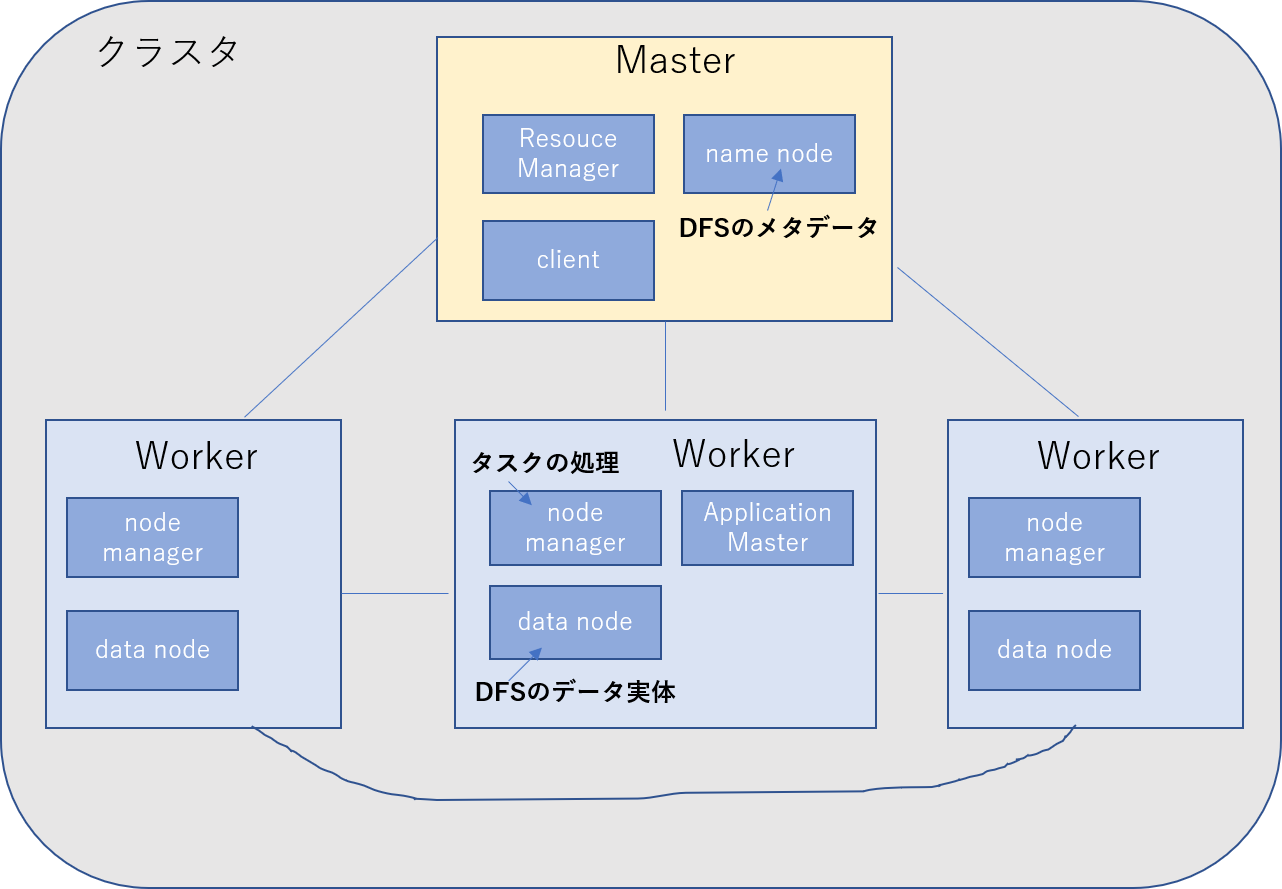
\includegraphics[scale=0.3]{figures/distributed-processing-system.png}
  \caption{分散処理フレームワーク概要図}
  \label{fig:ditributed-processing-system}
\end{figure}

\subsection{Apache Spark}
Apache Spark はインメモリ分散処理フレームワークの1 つで,分散処理フレームワークのなかでも
処理を出来る限りメモリ内で行うことでネットワークやI/O による遅延を防ぐことができる.Hadoop
などでは処理のたびにディスクアクセスが発生するため,ボトルネックが存在するという問題点がある.
Spark では処理後の一時データの出力先をディスクではなくメインメモリ
に書き出すことで,余計なディスクアクセスを減らしてHadoop の問題点を解決している.
また,ApacheSpark ではRDD\cite{zaharia2012resilient} とDAG\cite{dag} という仕組みが用いられており,処理のログを保存しておくことで,高い耐
障害性も維持している.これらのことから,分散処理フレームの中でも近年の主流となってきている.

\subsection{予備実験}
Apache Sparkへのヒュージページの効果を調査するために予備実験を行った.予備実験ではヒュージページの
割り当てをなし,全体への割り当て,StorageMemoryのみへの割り当てと3種類の状態で実験を行った.
実験結果を図\ref{fig:pre-experiment}に示す.
実験の結果ヒュージページはApache Sparkで効果的に働き実行時間を短縮させたことが分かった.また,
マイクロベンチマークやkmeansでは一部のメモリ割り当てでも全体割り当てに近い性能が得られることが分かった.
しかし,この一部割り当てを行うのはSparkからJNI\cite{jni}を通してmadviseシステムコール\cite{madvise}を呼び出すことによって,StorageMemoryのデータを
後からヒュージページに昇格していくという手法であり,ヒュージページになるのが遅く実行時間が短いと効果をあまり受けられないことや,メモリの
スキャンにオーバーヘッドがかかるという問題点が存在していた.

\begin{figure}
  \centering
  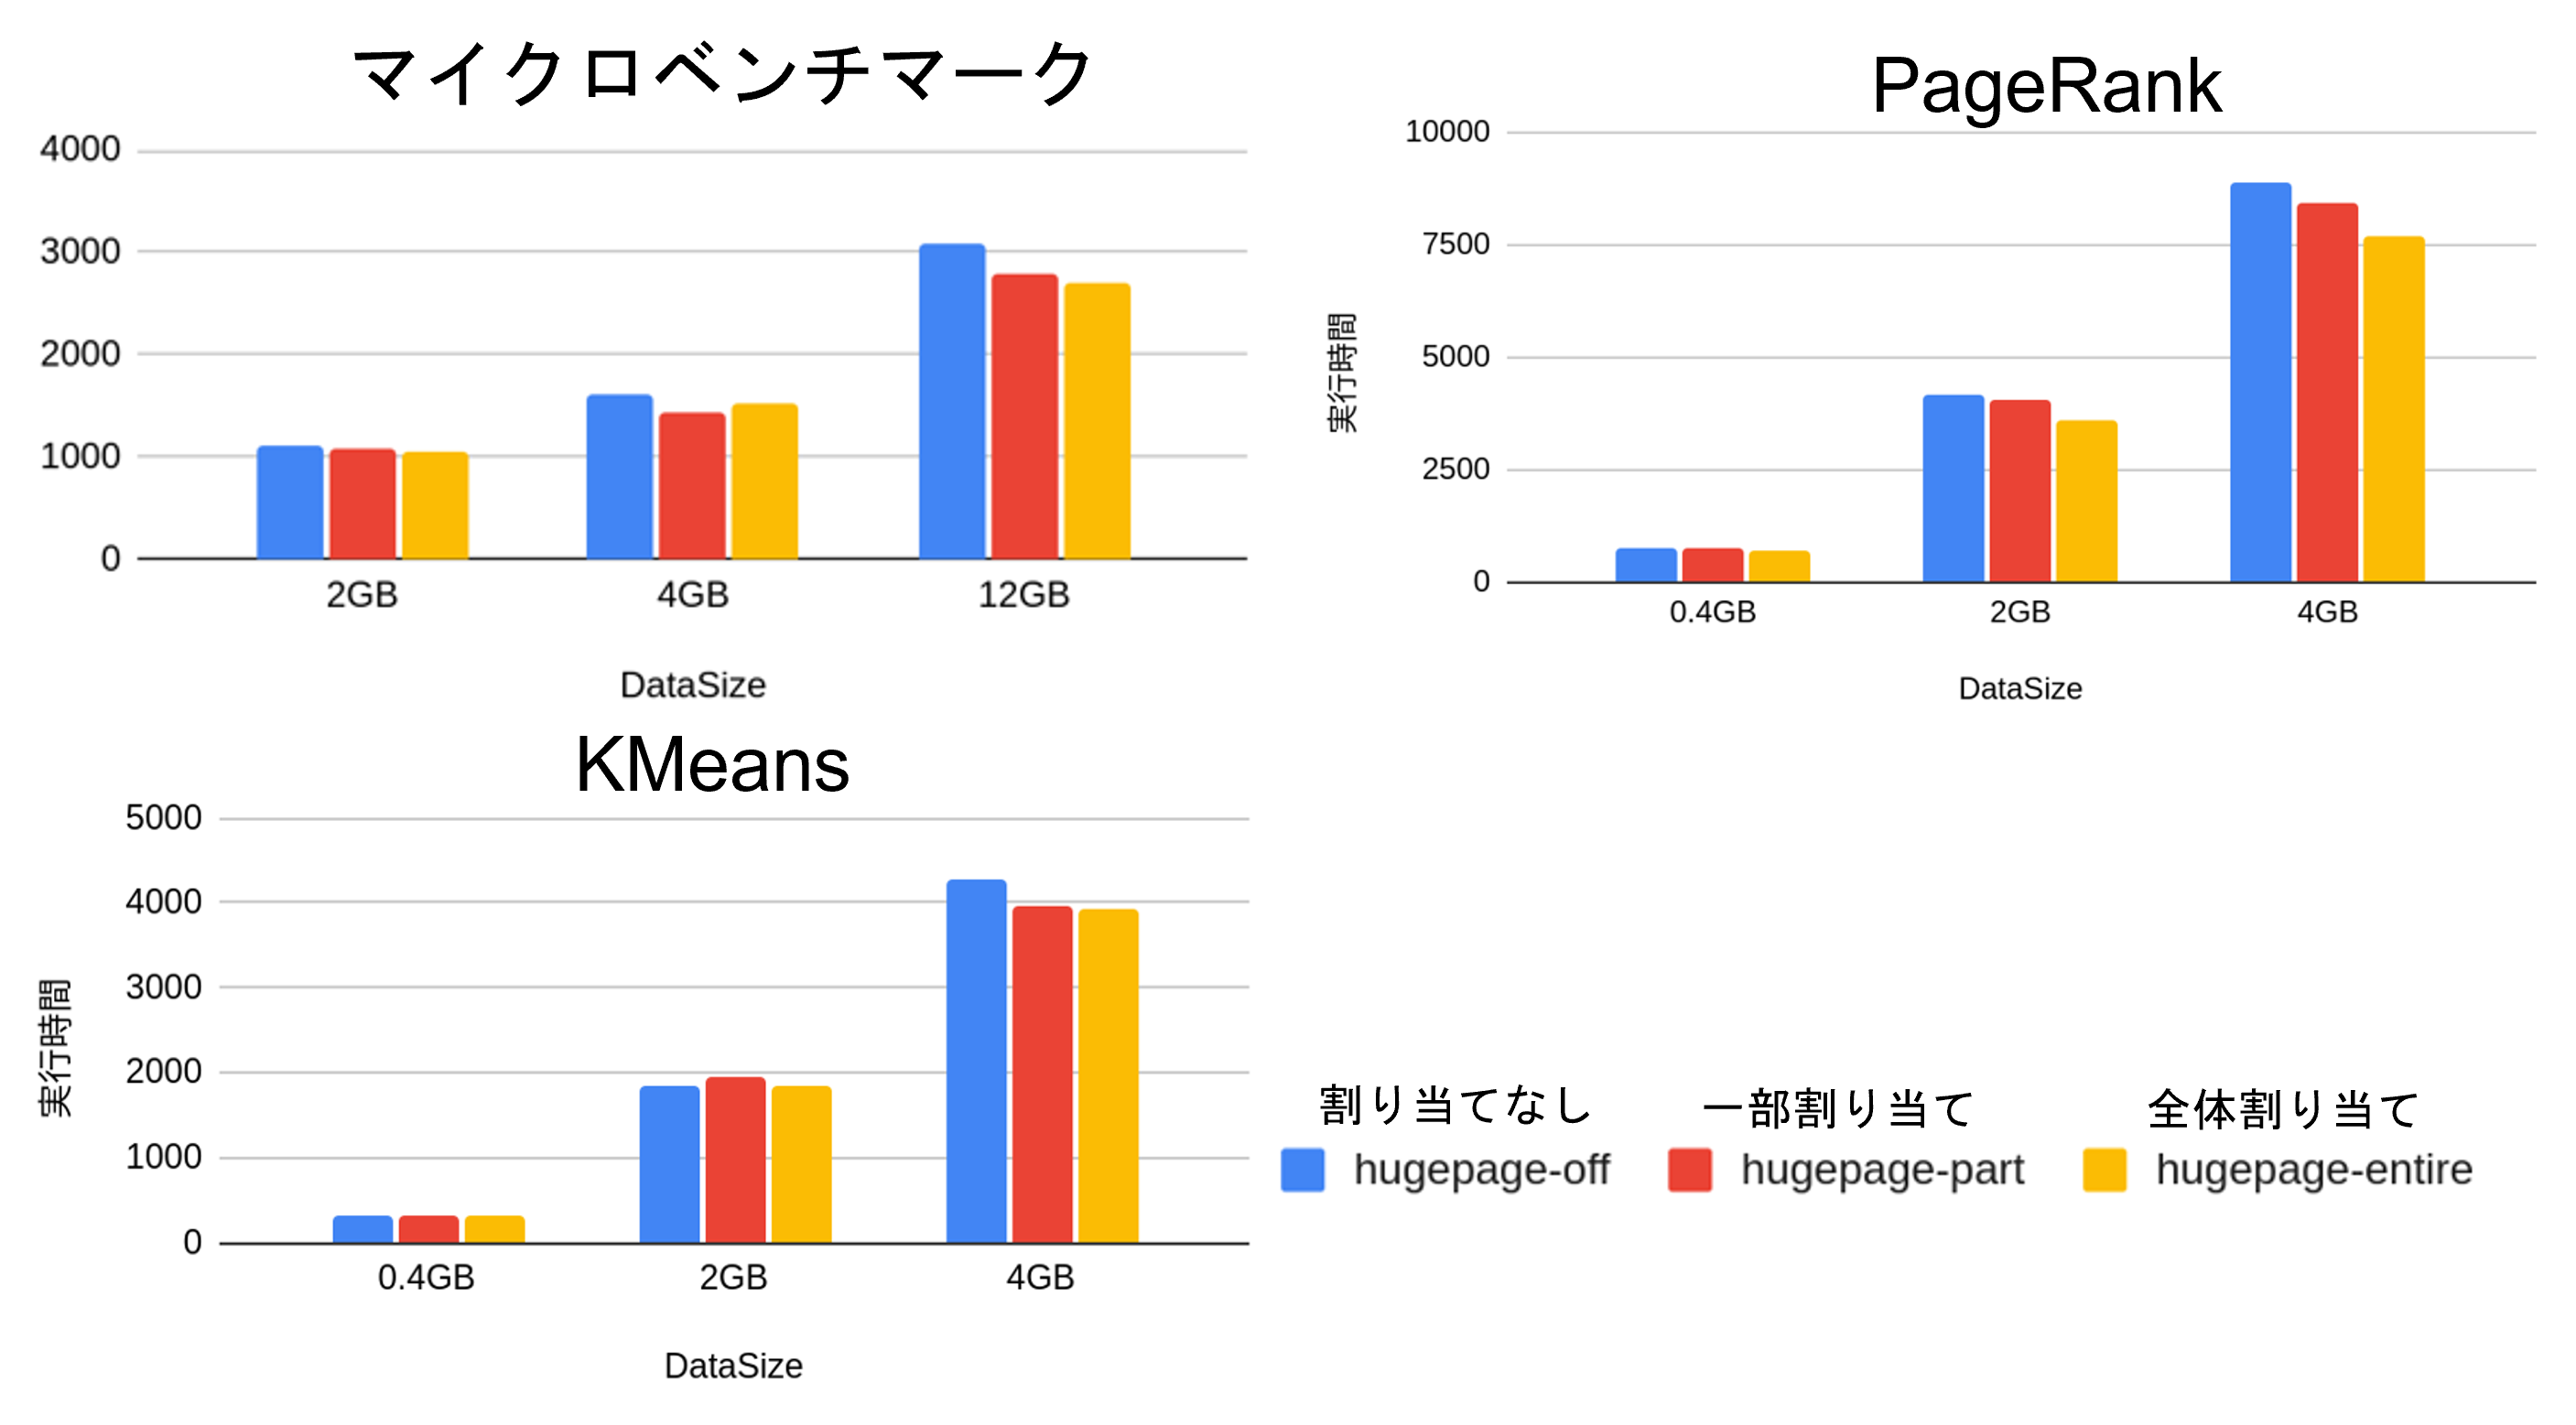
\includegraphics[scale=0.4]{figures/pre-experiment.png}
  \caption{予備実験結果}
  \label{fig:pre-experiment}
\end{figure}
\section{提案} \label{section:proposal}
本研究ではヒュージページを有効的に活用するインメモリ分散処理フレームワークを提案する.
アプローチとしてはヒュージページの効果を受けやすいようなデータはヒュージページで生成して,
それ以外は通常のページで割り当てすることで効率の良いヒュージページ割り当てを行う.
提案方式によってヒュージページの恩恵も受けつつもデメリットを最小限に抑えることができる.

提案を実現する際にデザインチャレンジとなるのが以下のものである.

\begin{itemize}
  \item \emph{ヒュージページの割り当てはアプリケーション単位でしか選択できない}\\
  Apache Sparkでヒュージページを使う際には実行時にJavaオプションでUseTransParentHugepagesを指定して実行する.
  そうするとTHPによってJVM全体がヒュージページに割当たることになる.この選択はJVMごとにしか選べないため
  データ単位で割り当てることが出来ずSparkの特性に適したデータごとの割り当てを行うことができない.
  そこでデータ単位でヒュージページ割り当てを行う手法が必要となってくる.
  \item \emph{ヒュージページの効果を受けやすい適したデータをどう選ぶか}\\
  データの一部をヒュージページに割り当てることが出来たとして,どのデータに割り当てすれば
  効率的にヒュージページが使えるかを考える必要がある.
\end{itemize}




\section{設計} \label{section:design}

\subsection{データ単位でのヒュージページ割り当て}
前章で述べた通り,Apache Sparkにおいてヒュージページを使う際にはアプリケーション単位でしか
使用の有無を選択できない.これはJVMのオプションとしてJVM全体にヒュージページを使うか使わないかしか
選べないからである.

予備実験ではデータ単位での割り当てを行うための実装をSparkにおいて行った.手法としてはStorageMemoryに
あるデータを定期的にスキャンし,1ページに一定以上のサイズが含まれている場合はヒュージページに昇格するように
マークをつけていくという方式となっている.これによって一部のヒュージページ割り当てには成功したが,
一度割り当てたデータを後から昇格するため昇格に時間がかかりヒュージページの効果が現れるのが遅いことや
メモリをスキャンするためにスレッドを一時停止するためオーバーヘッドが大きいといった問題点があった.

これらを解決するために今回の提案方式ではJVMに改良を加え,データごとにヒュージページを
使うかどうか選べるようにする.この改良されたJVMを使いSparkでデータを生成する際にそのデータの
特性に合わせてヒュージページを使うかどうか選ぶことで効率的なヒュージページ割り当てを行う.
JVM側でデータの生成の際に直接ヒュージページとして生成することで昇格を待つ必要がなく,すぐに
恩恵が受けられる.また,メモリをスキャンする必要がなくなったためオーバーヘッドを気にする
必要もなくなる.

\subsection{ヒュージページ割り当てを行うデータ}
Spark では図\ref{fig:spark-memory-management}に示すような形でメモリの管理が行われている\cite{spark-memory-management}.Reserved Memory はSpark 内
部オブジェクト用に確保された領域であり固定の大きさとなっている.User Memory はユーザデー
タ構造や内部メタデータを保存する領域である.Execution Memory はSpark のタスクを実行する
ためのメモリであり,主に短命なオブジェクトのための領域である.Storage Memory はキャッシュ
したRDD などが保存される領域で主に長命なオブジェクトを保存するための領域である.Storage
Memory とExecution Memory のサイズは明確に決まっておらず,状況によって領域が移動する.

Spark アプリケーションではファイルからデータをロードし,RDD としてStorage Memory に保存,
RDD へ繰り替えし処理を行う,という構成が多いため,Storage Memory には頻繁にアクセスされる
大きなデータが保存される.そのため,ヒュージページの影響を大きく受ける領域はStorage Memory
ではないかと考えられる.
よって提案方式ではこのStorageMemoryに保存されるデータに対してヒュージページ割り当てを行う.

\begin{figure}
  \centering
  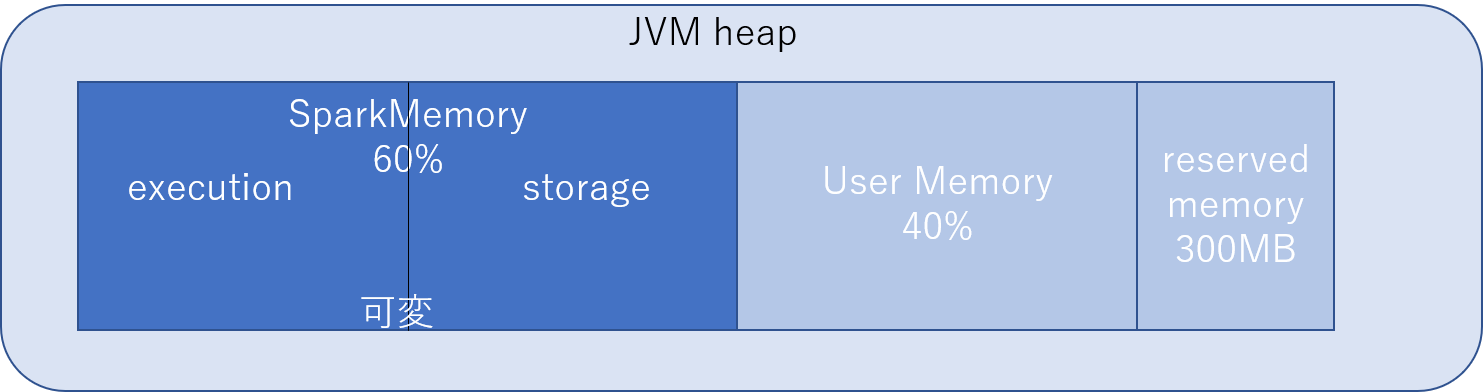
\includegraphics[scale=0.3]{figures/spark-memory-management.png}
  \caption{Sparkメモリ管理}
  \label{fig:spark-memory-management}
\end{figure}

\section{実装} \label{section:implementation}
本研究では,Apache Spark3.2とOpenJDK11\cite{open-jdk}を実装対象とし,OpenJDKにデータ単位でのヒュージページ割り当てを
行うための機能を追加し,Sparkにその機能を用いて繰り返し利用されるデータに対してヒュージページを
割り当てるように変更を行った.

\subsection{JVMの改良}
Javaではオブジェクトを生成する際にnew命令を使って生成を行う.このnew命令に加えてオブジェクトを生成する際に
ヒュージページで生成するhp\_new命令を実装した.また,配列を生成するnewarray命令などもあるため,それぞれの
生成命令にはヒュージページで生成する命令を実装している.
実装のためにまず,JVMにHugepageRegionを追加した.Openjdk11の標準GCであるG1GC\cite{detlefs2004garbage}ではメモリがRegionという単位で
分割され管理されており,HugepageRegionはこのRegionをヒュージページとしたものである.
hp\_new命令が初めて呼び出されると通常のRegionを保存するフリーリストの中から使用したことのない
Regionを選びHugepageRegion専用のフリーリストに移動する.
一度別の用途に使われた後にフリーリストに返されたRegionだとヒュージページを割り当てる際に直接
ヒュージページ割り当てが出来ず,昇格によってヒュージページになるため優先して使用したことのないRegionが
選択される.
選択されたRegionはmadviseシステムコールによってMADV\_HUGEPAGEアドバイスが追加される.これによりこのRegionに
メモリを割り当てる際にはヒュージページとして割り当てられるようになる.
以降はhp\_new命令が呼び出された時はHugepageRegionから割り当て,存在しない場合は同じようにフリーリストから
もらってくるという手順となっている.
また,HugepageRegionを返す場合はヒュージページ専用のフリーリストに返すことでヒュージページと通常のページの
分離を行っている.
これにより通常はnew命令による通常の割り当て,ヒュージページを使いたい時はhp\_new命令を使うことで
データ単位でヒュージページの使用の有無を選べるようになる.
また,追加の工夫としてHugepageRegionは最初からOld領域にするようにしている.HugepageRegionに保存されるデータは長期間利用されるのが
前提のため,最初からOld領域にすることでYoung領域でGCを何度もされてOld領域へ移動といった手間を省くことができる.

\subsection{Sparkの改良}
Spark側ではStorageMemoryのデータを生成する際にhp\_new命令を使う用にする.
ここでhp\_new命令を使うケースとして二つ存在している.
まず,StorageMemoryに保存したいオブジェクトを自身のコード内で生成している場合である.
このような場合はユーザがhp\_new命令をコード内で記述してヒュージページとしての生成を行うことになる.
これによりhp\_new命令を使用したオブジェクトがヒュージページに割当たるようになる.
2つ目のケースがファイルなどに保存しておいたデータをシリアライズしてStorageMemoryにRDDとして保存する
場合である.このケースではSpark内でデータをキャッシュする際に利用するバッファーの生成に
hp\_newを使うようになっている.このバッファーがヒュージページで確保されることでデータがヒュージページとして
割当たることになる.
この場合ではユーザがコードの変更をすることなくStorageMemoryのデータをヒュージページとして割り当てることができる.




\section{実験} \label{section:evaluation}
提案方式によるヒュージページ割り当てとヒュージページなし,標準のヒュージページ割り当て(全体割り当て),
予備実験での手法でのヒュージページ割り当てと4つのヒュージページ割り当ての方法の4つのヒュージページ割り当てポリシーで実験を行った.
実験では実行時間やヒュージページ割り当てサイズ,TLBミス率などを計測した.TLBミスの計測にはperf\cite{perf}コマンドを用いている.
実験には作成した単純なマイクロベンチマークを利用した.マイクロベンチマークはStorageMemoryにデータをキャッシュし
そのデータに対してアクセスを繰り返すStorageMemoryへの負荷が大きい反復ワークロードとなっている.

\subsection{目的}
本実験の目的は提案方式が正しく機能し,一部への割り当てだけでも全体の割り当てと同等にヒュージページの恩恵を
受けられることを確認する.
また,今回の提案方式では予備実験で使用した手法のデメリットが解消されていることも確認する.

\subsection{実験環境}
実験で使用したマシンの性能を表\ref{tab:master-node}に,Sparkの設定を表\ref{tab:spark-config}に示す.実験ではワーカーノードを2つ用意し,各ワーカーノード内で2つのエグゼキュータを起動することで,合計4つのエグゼキュータを動かしている.
また、リソースマネージャーとしてHadoop YARN\cite{vavilapalli2013apache}を利用する。
\begin{table}
	\caption{マシン性能}
	\label{tab:master-node}
	\centering
	\begin{tabular}{ccc}
		\hline
		 & マスターノード & ワーカーノード \\
		\hline
		CPU & Intel Xeon E5-2430 v2 & Intel Xeon E-2124 \\
		\hline
		コア数 & 4 & 4 \\
		\hline
		RAM & 32 & 64 \\
		\hline
		kernel & 5.4.0 & 5.4.0\\
		\hline
	\end{tabular}
\end{table}
\begin{table}
	\caption{Sparkの設定}
	\label{tab:spark-config}
	\centering
	\begin{tabular}{cc}
		\hline
		エグゼキュータ数 & 4 \\
		\hline
		コア数 & 1 \\
		\hline
		メモリ & 20GB \\
		\hline
	\end{tabular}
\end{table}

\subsection{実行時間}
実行時間を図\ref{fig:storagememory-exec-100000}に示す.
2GBのようにデータサイズが小さい時は実行時間に対してメモリアクセスの時間が少ないためどの条件でも大きな差はない.
4GB, 12GBだと差が表れてきており,今回の提案方式(hugepage-part)>全体割り当て(hugepage-entire)
>予備実験での手法(hugepage-part-old)>割り当てなし(hugepage-off)の順番に早くなっていることが分かる.
今回の提案方式が一番早くなっており,これはヒュージページの恩恵は全体割り当てと同様に受けているのに加えて
メモリコンパクションなどのヒュージページのデメリットは抑えられたことが原因だと考えられる.
また,最初からOld領域に割り当てることによるGCの節約も原因の一つだと考えられる.
予備実験での手法では実行時間の削減ができてはいるが,他の割り当てありに劣り,ヒュージページを使うのが
遅いことやメモリスキャンオーバーヘッドが出ているとわかる.今回の方式では全体割り当て以上に削減できており
その問題点を改善としていることがわかる.

\begin{figure}[H]
  \centering
  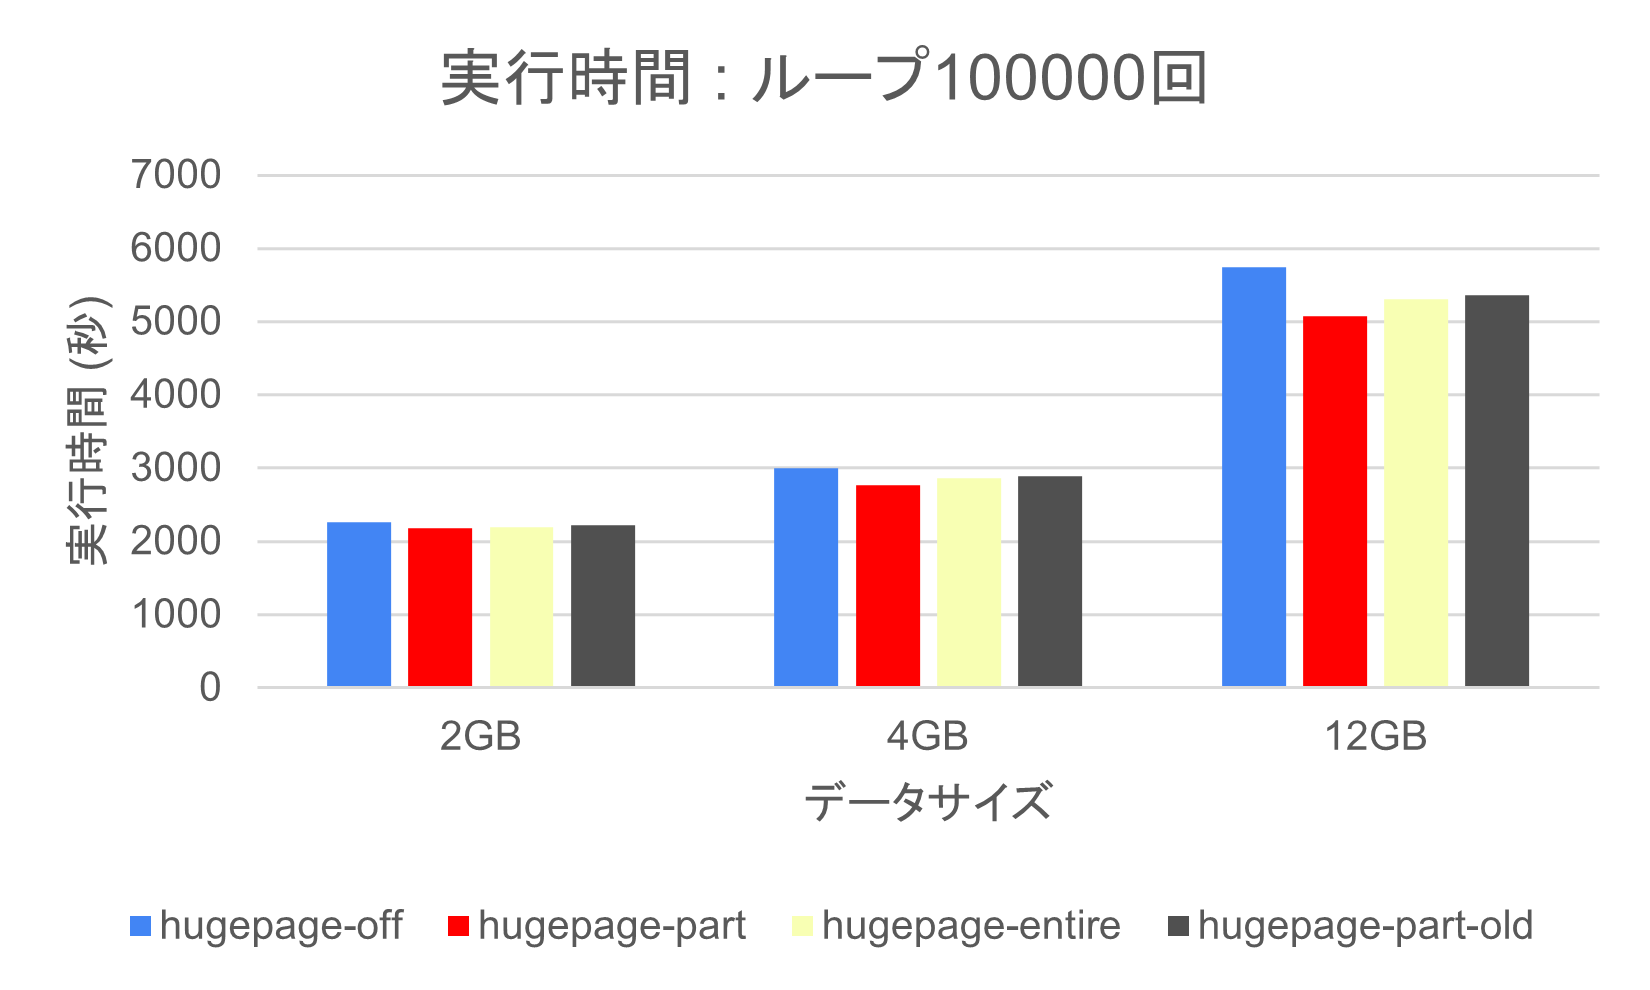
\includegraphics[scale=0.6]{figures/experiment-new/storagememory/exec-100000.png}
  \caption{実験結果:実行時間}
  \label{fig:storagememory-exec-100000}
\end{figure}

\subsection{TLBミス率}
TLBミス率を図\ref{fig:storagememory-tlb-miss-100000}に示す
全体割り当て,今回の提案方式が両方とも大きくTLBミス率を削減しており,このTLBミスの削減で実行時間が削減されたと分かる.
予備実験の手法は他よりも削減率が良くないことからヒュージページを使い始めるのが遅く恩恵を十分に受けられていないことが分かる.
対して今回の提案方式は全体割り当てに近く大幅なTLBミス率の削減ができているので,ヒュージページを最初から
十分に使えているとわかる.

\begin{figure}
  \centering
  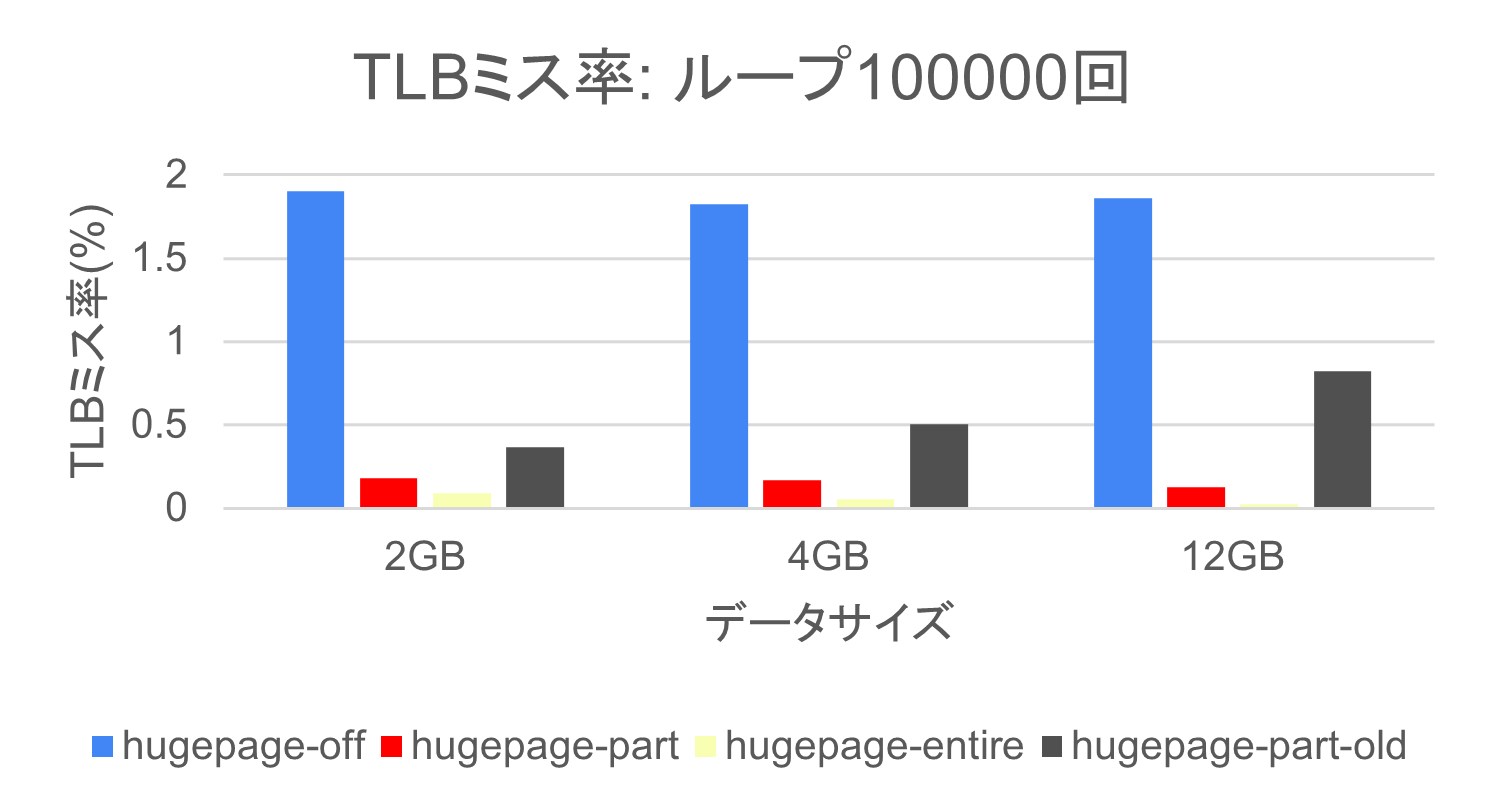
\includegraphics[scale=0.6]{figures/experiment-new/storagememory/tlb-miss-100000.png}
  \caption{実験結果:TLBミス率}
  \label{fig:storagememory-tlb-miss-100000}
\end{figure}

\subsection{ヒュージページ割り当て数の比較}
データサイズ12GBでのヒュージページ割り当て数の遷移を図\ref{fig:storagememory-throughput-hugepage-4g-100000}に示す.
今回の提案方式では即座に3GBの割り当てを行っている.サイズとして4つのExecutorが12GBをそれぞれ保存するため,
12/4 = 3GBのデータであり,StorageMemoryのデータをすぐに全部割り当てることができている.
予備実験の方式では割り当てに長い時間がかかっており,ヒュージページの恩恵を十全に受けられるまで時間が
かかっているのがわかる.
全体割り当てについてはStorageMemroy以外のデータにも割り当てを行っており,ヒュージページを使うサイズが
大きくなっている.この時の無駄な割り当てによるオーバーヘッドが実行時間に出てきていると考えられる.

\begin{figure}[H]
  \centering
  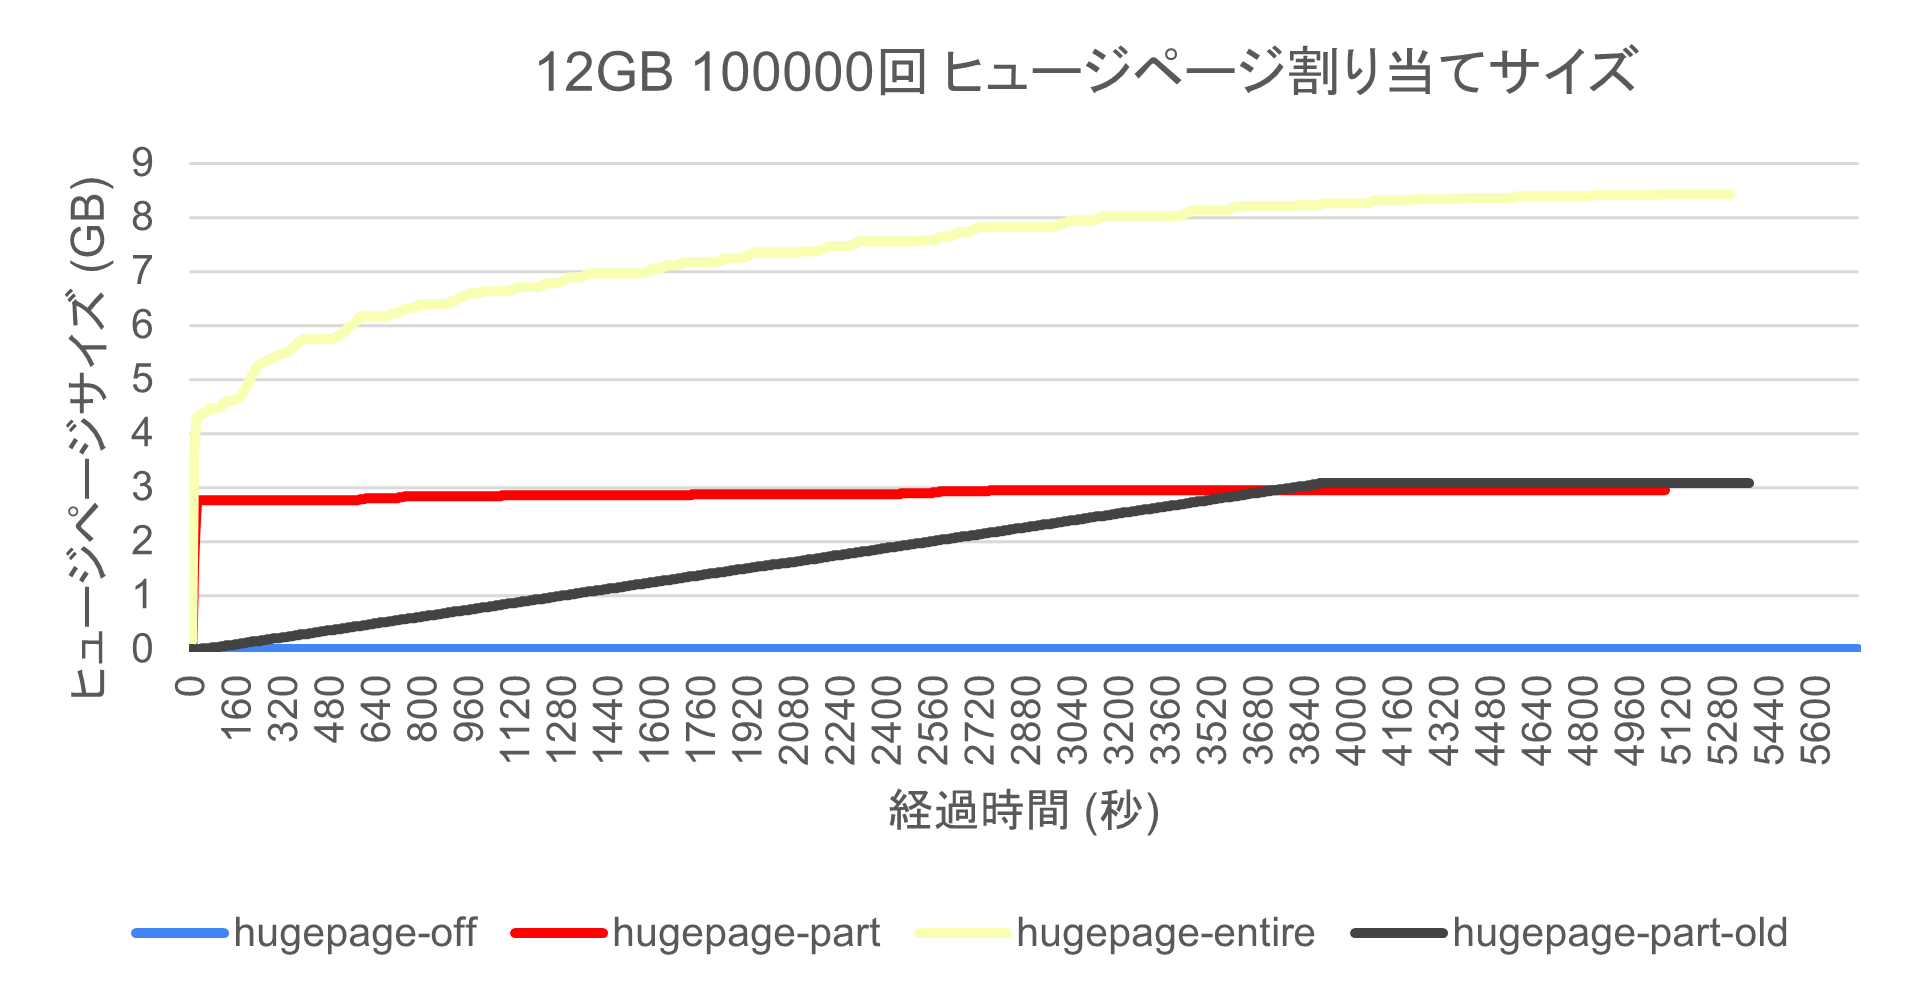
\includegraphics[scale=0.5]{figures/experiment-new/storagememory/throughput-hugepage-4g-100000.png}
  \caption{実験結果:ヒュージページ割り当てサイズ}
  \label{fig:storagememory-throughput-hugepage-4g-100000}
\end{figure}

\section{関連研究}
HotTub\cite{lion2016don}はJVMのウォームアップ時間を減らすことで分散処理フレームワークのパフォーマンスを向上させる
機構である.HotTubではJVMのウォームアップを減らすためにJVMの再利用を行う.一度使用したJVMは
通常そのまま終了されるところを一旦プールしておき,他のアプリケーションによってJVMを起動する時に
プールしておいたJVMを再利用することでウォームアップにかかる時間を短縮する.
結果としてHotTubはウォームアップ時間を短縮し,HDFS\cite{shvachko2010hadoop}の読み書きやSparkSQL\cite{armbrust2015spark}などのワークロードでの実行時間の
短縮に成功している.

Yak\cite{nguyen2016yak}は分散処理システムに適したGCで世代別GCと領域ベースのGCを組み合わせたものとなる.
YakではSparkのオブジェクト特性に注目し,オブジェクトが長寿でライフサイクルが同じであるという
ことを利用して,オブジェクト適正に合わせたGCを行うことでGC時間を短縮させている

Riffle\cite{zhang2018riffle}はMapReduceのシャッフルフェーズにオーバーヘッドが大きいことに注目し,シャッフルの際の
細かい中間データをマージして一つにすることでシャッフル時間を短縮させることに成功している.

Ingens\cite{kwon2016coordinated}はTHPの問題点を解決し効率的なヒュージページ管理を行う機構である.Ingensではヒュージページの
使用率とアクセス頻度を監視し,その情報をもとに適切なタイミングでヒュージページ割り当てを行うことで
断片化の解消やメモリの節約といったパフォーマンスの向上を行っている.

Illuminator\cite{panwar2018making}はTHPのメモリ汚染による断片化を減らし,効率的なヒュージページ管理を行う機構である.
IlluminatorではLinuxに存在するユーザ用の移動可能なmovableとカーネル用の移動不可能なunmvableな
メモリ領域に加えてmovableとunmovableが混在したハイブリッド領域を明示的に管理し,ハイブリッド
領域ではヒュージページ割り当てを避けることで無駄にページ移動することを防いでいる.
結果としてIlluminatorはページ移動にかかる時間を短縮させ,パフォーマンスを向上させている.

これらの研究はヒュージページと分散処理フレームワークそれぞれに個別に対処したものであり,
インメモリ分散処理フレームワークを対象としたヒュージページ割り当てに関する研究は行われていない.
本研究では分散処理フレームワーク固有の特性を考慮して効率的にヒュージページを利用する
手法を提案した.
\section{おわりに} \label{section:conclusion}
本研究ではヒュージページを活用するインメモリ分散処理フレームワークを提案した.
ヒュージページはインメモリ分散処理フレームワークのような膨大なメモリを利用するアプリケーションと
相性がよくパフォーマンスの向上が期待できる.
しかし,現在インメモリ分散処理フレームワークでヒュージページを使うにはアプリケーション単位でしか
選択できず,データ単位で割り当てることができない.
THPにはメモリ肥大化やメモリコンパクションのためのCPU占有などのデメリットが存在するため
闇雲にアプリケーション全体に割り当てるのが正しいとは限らず,Sparkのデータ特性に合わせた
割り当てが必要となってくる.
提案方式ではデータ単位でのヒュージページ割り当てを実装し,長期間生存して再利用されやすい
データに対してのみヒュージページ割り当てを行うことで,ヒュージページの恩恵を受けつつ,デメリットを抑えることを狙う.
提案方式をApache SparkとOpenJDKに実装しマイクロベンチマークで実験を行った.
実験の結果,実装したシステムが正常に動作し,一部のメモリにのみヒュージページを割り当てることに
成功した.そして,提案方式が全体割り当てよりも実行時間を削減できたことを確認した.
今後として,マイクロベンチマーク以外のPagerank\cite{page1999pagerank}やkmeansといったReal-timeなワークロードの
実験を行う.また,提案方式ではユーザが自身のコード内で生成したオブジェクトをヒュージページに
するためにはコードをユーザが変更する必要があった.既存のコードの再利用などのために,
StrageMmeoryにキャッシュされるオブジェクトについては全てを自動でヒュージページにするように
改良を行う必要があると考えられる.




\bibliographystyle{ipsjunsrt}
\bibliography{references}


\end{document}
